% Created 2019-11-19 火 10:29
% Intended LaTeX compiler: pdflatex
\documentclass[presentation,dvipdfmx,CJKbookmarks]{beamer}
\usepackage{CJKutf8}
\usepackage{atbegshi}
\AtBeginShipoutFirst{\special{pdf:tounicode UTF8-UTF16}} % for UTF-8
\usepackage[utf8]{inputenc}
\usepackage[T1]{fontenc}
\usepackage{graphicx}
\usepackage[export]{adjustbox}
\usepackage{lmodern}
\usepackage{grffile}
\usepackage{longtable}
\usepackage{wrapfig}
\usepackage{rotating}
\usepackage[normalem]{ulem}
\usepackage{amsmath}
\usepackage{textcomp}
\usepackage{amssymb}
\usepackage{capt-of}
\usepackage{hyperref}
 \usepackage{minted}
\usetheme{Berkeley}
\usecolortheme{lily}
\author{[锤子科技 smartisan] 包昊军}
\date{2017-05-08}
\title{\text{\includegraphics[width=1em,valign=t,raise=0.1em,natwidth=48bp,natheight=48bp]{/home/bhj/src/github/Wrench/release/emojis/iphone-new/PERSONAL_COMPUTER.png}}、\text{\includegraphics[width=1em,valign=t,raise=0.1em,natwidth=48bp,natheight=48bp]{/home/bhj/src/github/Wrench/release/emojis/iphone-new/MOBILE_PHONE.png}}、\text{\includegraphics[width=1em,valign=t,raise=0.1em,natwidth=48bp,natheight=48bp]{/home/bhj/src/github/Wrench/release/emojis/iphone-new/WRENCH.png}}}
\hypersetup{
 pdfauthor={[锤子科技 smartisan] 包昊军},
 pdftitle={\text{\includegraphics[width=1em,valign=t,raise=0.1em,natwidth=48bp,natheight=48bp]{/home/bhj/src/github/Wrench/release/emojis/iphone-new/PERSONAL_COMPUTER.png}}、\text{\includegraphics[width=1em,valign=t,raise=0.1em,natwidth=48bp,natheight=48bp]{/home/bhj/src/github/Wrench/release/emojis/iphone-new/MOBILE_PHONE.png}}、\text{\includegraphics[width=1em,valign=t,raise=0.1em,natwidth=48bp,natheight=48bp]{/home/bhj/src/github/Wrench/release/emojis/iphone-new/WRENCH.png}}},
 pdfkeywords={},
 pdfsubject={},
 pdfcreator={Emacs 26.3 (Org mode 9.1.9)},
 pdflang={English}}
\begin{document}
\begin{CJK*}{UTF8}{simsun}

\maketitle
\begin{frame}{Outline}
\tableofcontents
\end{frame}

\CJKtilde

\section{什么是小扳手?}
\label{sec:org4231762}

\begin{frame}[label={sec:org6af7f41}]{在\text{\includegraphics[width=1em,valign=t,raise=0.1em,natwidth=48bp,natheight=48bp]{/home/bhj/src/github/Wrench/release/emojis/iphone-new/DESKTOP_COMPUTER.png}}上连接、操作安卓\text{\includegraphics[width=1em,valign=t,raise=0.1em,natwidth=48bp,natheight=48bp]{/home/bhj/src/github/Wrench/release/emojis/iphone-new/MOBILE_PHONE.png}}}
\begin{block}{把\text{\includegraphics[width=1em,valign=t,raise=0.1em,natwidth=48bp,natheight=48bp]{/home/bhj/src/github/Wrench/release/emojis/iphone-new/MOBILE_PHONE.png}}变得像\text{\includegraphics[width=1em,valign=t,raise=0.1em,natwidth=48bp,natheight=48bp]{/home/bhj/src/github/Wrench/release/emojis/iphone-new/PERSONAL_COMPUTER.png}}上的[QQ]一样方便}
\begin{itemize}
\item 在\text{\includegraphics[width=1em,valign=t,raise=0.1em,natwidth=48bp,natheight=48bp]{/home/bhj/src/github/Wrench/release/emojis/iphone-new/PERSONAL_COMPUTER.png}}上接收\text{\includegraphics[width=1em,valign=t,raise=0.1em,natwidth=48bp,natheight=48bp]{/home/bhj/src/github/Wrench/release/emojis/iphone-new/MOBILE_PHONE.png}}聊天消息、弹窗通知
\item 在\text{\includegraphics[width=1em,valign=t,raise=0.1em,natwidth=48bp,natheight=48bp]{/home/bhj/src/github/Wrench/release/emojis/iphone-new/PERSONAL_COMPUTER.png}}上输入文字、表情符,通过\text{\includegraphics[width=1em,valign=t,raise=0.1em,natwidth=48bp,natheight=48bp]{/home/bhj/src/github/Wrench/release/emojis/iphone-new/MOBILE_PHONE.png}}发送
\item 发送图片
\item 自动抢[微信]、[QQ]红包
\item 个性化定制
\end{itemize}
\end{block}

\begin{block}{自动化操作\text{\includegraphics[width=1em,valign=t,raise=0.1em,natwidth=48bp,natheight=48bp]{/home/bhj/src/github/Wrench/release/emojis/iphone-new/MOBILE_PHONE.png}}}
\begin{itemize}
\item [微信]、[QQ空间]、[微博]社交软件上的分享
\item 一键扫码
\item 搜索联系人、[亚马逊 Kindle]电子书
\end{itemize}
\end{block}

\begin{block}{谁适合用\text{\includegraphics[width=1em,valign=t,raise=0.1em,natwidth=48bp,natheight=48bp]{/home/bhj/src/github/Wrench/release/emojis/iphone-new/WRENCH.png}}[疑问]}
\end{block}
\end{frame}
\section{屏幕同步}
\label{sec:org04f8cf3}
\begin{frame}[label={sec:org1cd0b5d}]{演示模式:小扳手发布会\text{\includegraphics[width=1em,valign=t,raise=0.1em,natwidth=48bp,natheight=48bp]{/home/bhj/src/github/Wrench/release/emojis/iphone-new/WHITE_SMILING_FACE.png}}}
\begin{center}
\includegraphics[width=.9\linewidth]{./images/wrench-demo.ps}
\end{center}
\end{frame}

\section{\text{\includegraphics[width=1em,valign=t,raise=0.1em,natwidth=48bp,natheight=48bp]{/home/bhj/src/github/Wrench/release/emojis/iphone-new/WRENCH.png}}\text{\includegraphics[width=1em,valign=t,raise=0.1em,natwidth=48bp,natheight=48bp]{/home/bhj/src/github/Wrench/release/emojis/iphone-new/ELECTRIC_LIGHT_BULB.png}}演示}
\label{sec:orgfe5271c}
\begin{frame}[label={sec:org4bcc0bb}]{聊天和分享}
\begin{block}{查找联系人}
\end{block}
\begin{block}{文字、表情符的输入、发送\text{\includegraphics[width=1em,valign=t,raise=0.1em,natwidth=48bp,natheight=48bp]{/home/bhj/src/github/Wrench/release/emojis/iphone-new/FACE_WITH_ROLLING_EYES.png}}[doge]}
\end{block}
\begin{block}{接收、处理聊天消息}
\end{block}
\begin{block}{发送图片\text{\includegraphics[width=1em,valign=t,raise=0.1em,natwidth=48bp,natheight=48bp]{/home/bhj/src/github/Wrench/release/emojis/iphone-new/FRAME_WITH_PICTURE.png}}}
\begin{itemize}
\item 从浏览器直接拖图(像不像[一步][疑问])
\end{itemize}
\end{block}
\begin{block}{分享到[微博]、[微信]、[QQ空间]}
\end{block}
\end{frame}


\begin{frame}[label={sec:org9a12964}]{搜索}
\begin{block}{找[微信]联系人}
\end{block}
\begin{block}{找[QQ]联系人}
\end{block}
\begin{block}{找[QQ]群里的联系人}
\end{block}
\begin{block}{找[微博]上的用户}
\end{block}
\begin{block}{按发件人找[邮件]}
\end{block}
\begin{block}{在[亚马逊 Kindle]里搜书}
\end{block}
\end{frame}

\begin{frame}[label={sec:orgffe710a}]{扫码}
\begin{block}{[微信]扫码}
\end{block}
\begin{block}{[微博]扫码}
\end{block}
\begin{block}{[手机京东]扫码}
\end{block}
\begin{block}{自动登录微信公众号的\thinspace system-config\thinspace 脚本演示}
\end{block}
\end{frame}

\begin{frame}[label={sec:org07b704c}]{抢红包}
\begin{block}{抢[微信]红包(并自动表示\text{\includegraphics[width=1em,valign=t,raise=0.1em,natwidth=48bp,natheight=48bp]{/home/bhj/src/github/Wrench/release/emojis/iphone-new/PERSON_BOWING_DEEPLY.0.png}})}
\end{block}
\begin{block}{抢[QQ]红包}
\end{block}
\end{frame}

\section{高级用法}
\label{sec:orge4938d2}
\begin{frame}[label={sec:orgb8d8c67}]{自己录制控制手机的\thinspace Lua\thinspace 脚本}
\begin{block}{用鼠标右键点击屏幕同步窗口}
\begin{center}
\includegraphics[width=.9\linewidth]{./images/wrench-screen-record.ps}
\end{center}
\end{block}
\end{frame}

\section{开源信息}
\label{sec:org9706b3a}
\begin{frame}[label={sec:org4a60009}]{\text{\includegraphics[width=1em,valign=t,raise=0.1em,natwidth=48bp,natheight=48bp]{/home/bhj/src/github/Wrench/release/emojis/iphone-new/WRENCH.png}}是开源项目}
\begin{block}{项目\thinspace github\thinspace 网址}
\url{https://github.com/SmartisanTech/Wrench}
\end{block}

\begin{block}{使用\thinspace Qt、Lua\thinspace 编程,支持所有主流\thinspace PC\thinspace 平台}
\begin{itemize}
\item Linux
\item Mac
\item Windows
\end{itemize}
\end{block}

\begin{block}{支持几乎所有安卓手机}
\begin{itemize}
\item 支持[锤子科技 smartisan]所有机型
\item 其他厂商手机最低安卓版本要求请参考\thinspace Smartisan T1
\end{itemize}
\end{block}
\end{frame}

\begin{frame}[label={sec:org3042fe3}]{下载、文档}
\begin{block}{下载地址}
\href{https://github.com/SmartisanTech/Wrench-releases/releases}{Github SmartisanTech Wrench-Releases}
\end{block}

\begin{block}{使用手册}
\href{http://baohaojun.github.io/blog/2014/12/01/0-T1Wrench-2.0-Usage-Guide.html}{博客文章《小扳手使用手册》}
\end{block}

\begin{block}{开发手册}
Github Project Readme
\end{block}
\end{frame}

\begin{frame}[label={sec:orga2ce8e3}]{致谢、How to Help}
\begin{block}{致谢}
\begin{itemize}
\item [锤子科技 smartisan] \href{http://www.smartisan.com/cn/}{锤子科技}
\end{itemize}
\end{block}
\begin{block}{Help \text{\includegraphics[width=1em,valign=t,raise=0.1em,natwidth=48bp,natheight=48bp]{/home/bhj/src/github/Wrench/release/emojis/iphone-new/WRENCH.png}} Project}
\begin{itemize}
\item 源代码\thinspace Patch、[瓢虫]修正
\item 购买、使用锤子科技手机
\item 求转发[求关注]、帮助更多朋友使用小扳手
\item 用小扳手给作者打钱[疑问][捂脸][机智]
\item 微信公众号: Programate
\end{itemize}
\end{block}
\end{frame}

\section{\text{\includegraphics[width=1em,valign=t,raise=0.1em,natwidth=48bp,natheight=48bp]{/home/bhj/src/github/Wrench/release/emojis/emojione-v2.2.6-22/EGG.png}}高清阅读模式}
\label{sec:orgf597348}
\begin{frame}[label={sec:org111f9b2}]{在手机上沉浸式阅读电子书}
\begin{center}
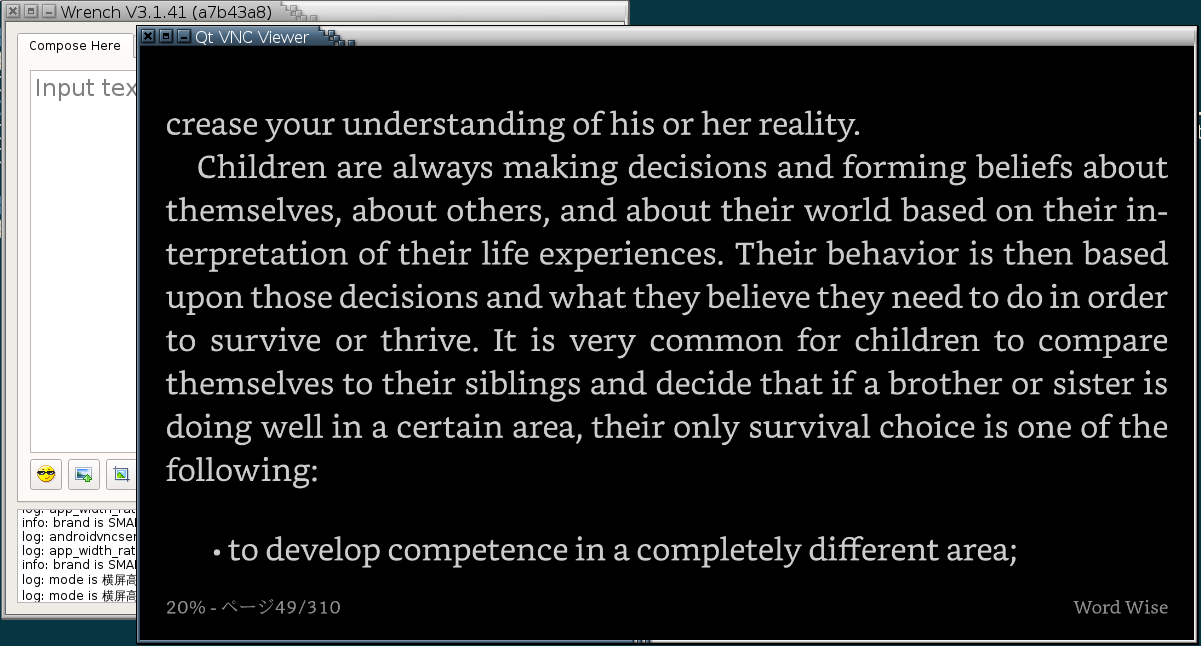
\includegraphics[width=.9\linewidth]{./images/wrench-read.ps}
\end{center}
\end{frame}

\begin{frame}[label={sec:org635bb96}]{Why[疑问]}
\begin{block}{手机上看书太\text{\includegraphics[width=1em,valign=t,raise=0.1em,natwidth=48bp,natheight=48bp]{/home/bhj/src/github/Wrench/release/emojis/iphone-new/TIRED_FACE.png}}了!}
\end{block}
\begin{block}{手机上看书太容易\text{\includegraphics[width=1em,valign=t,raise=0.1em,natwidth=48bp,natheight=48bp]{/home/bhj/src/github/Wrench/release/emojis/iphone-new/BROKEN_HEART.png}}了!}
\begin{itemize}
\item 一不小心就把[微博]打开
\item 一不小心就把[微信]朋友圈打开
\end{itemize}
\end{block}
\begin{block}{不是有网页版\thinspace Kindle Reader\thinspace 吗?}
\begin{itemize}
\item 跟手持\thinspace Kindle\thinspace 设备间的不同步问题[吐][衰]
\end{itemize}
\end{block}
\begin{block}{跟\thinspace \href{https://github.com/baohaojun/system-config}{system-config}\thinspace 结合,手机上的金山词霸[鼓掌]}
\end{block}
\end{frame}
\end{CJK*}
\end{document}
